\documentclass[border=1pt]{standalone}
% ---------------------------------------------------------------------------
% Shared style for the MOSAIC / CRYSTAL TOMM figures.
% Compile each fig_*.tex with LuaLaTeX (standalone). Sized for acmart
% "acmsmall" (TOMM): \textwidth = 13.9 cm, so every figure is drawn at
% final size and is included with width=\textwidth (no rescaling of text).
% Fonts: Libertinus Sans + Inconsolata (acmart uses Libertine + Inconsolata).
% ---------------------------------------------------------------------------
\usepackage{fontspec}
\setmainfont{LibertinusSans}[Path=fonts/, Extension=.otf,
  UprightFont=*-Regular, BoldFont=*-Bold, ItalicFont=*-Italic]
\setmonofont{Inconsolata}[Path=fonts/, Extension=.otf,
  UprightFont=*-Regular, BoldFont=*-Bold, Scale=0.98]
\usepackage{unicode-math}
\setmathfont{LibertinusMath-Regular.otf}[Path=fonts/]

\usepackage{tikz}
\usetikzlibrary{positioning,fit,calc,arrows.meta,backgrounds,
  shapes.misc,shapes.geometric,decorations.pathreplacing,patterns.meta}

% Okabe-Ito palette (colour-blind safe) + tints -------------------------------
\definecolor{oiBlue}{HTML}{0072B2}
\definecolor{oiOrange}{HTML}{E69F00}
\definecolor{oiSky}{HTML}{56B4E9}
\definecolor{oiGreen}{HTML}{009E73}
\definecolor{oiVerm}{HTML}{D55E00}
\definecolor{oiPurple}{HTML}{CC79A7}
\definecolor{oiYellow}{HTML}{F0E442}
\definecolor{ink}{HTML}{1A1A1A}
\definecolor{muted}{HTML}{5C5C5C}
\definecolor{rule}{HTML}{9A9A9A}

\definecolor{oursFill}{HTML}{DDEBF7}
\definecolor{oursDraw}{HTML}{0072B2}
\definecolor{modFill}{HTML}{FCEFD2}
\definecolor{modDraw}{HTML}{B57600}
\definecolor{upFill}{HTML}{F1F1F1}
\definecolor{upDraw}{HTML}{7D7D7D}
\definecolor{failFill}{HTML}{FBE3D6}
\definecolor{okFill}{HTML}{D9F0E8}

% Sequence colours (as in the packetization study)
\definecolor{seqSOL}{HTML}{0072B2}
\definecolor{seqTHA}{HTML}{009E73}
\definecolor{seqLON}{HTML}{CC79A7}

% Typography -----------------------------------------------------------------
\newcommand{\figfont}{\fontsize{7.5}{9}\selectfont}
\newcommand{\smallfig}{\fontsize{6.5}{7.8}\selectfont}
\newcommand{\tinyfig}{\fontsize{6}{7.2}\selectfont}
\newcommand{\code}[1]{{\ttfamily #1}}

% Provenance encoding: colour AND line style (grayscale safe) ------------------
%  ours      = new component written by us      (blue, solid 0.9 pt)
%  modified  = upstream component we patched    (orange, dashed 0.8 pt)
%  upstream  = used unmodified / third party    (grey, solid 0.45 pt)
\tikzset{
  base/.style={rectangle, rounded corners=1.6pt, align=center,
    inner xsep=3pt, inner ysep=2.6pt, font=\figfont, text=ink,
    execute at begin node={\hyphenpenalty=10000\exhyphenpenalty=10000}},
  ours/.style={base, fill=oursFill, draw=oursDraw, line width=0.9pt},
  mod/.style={base, fill=modFill, draw=modDraw, line width=0.8pt,
    dash pattern=on 2.6pt off 1.4pt},
  up/.style={base, fill=upFill, draw=upDraw, line width=0.45pt},
  dead/.style={base, fill=white, draw=oiVerm, line width=0.6pt,
    dash pattern=on 1.2pt off 1.2pt, text=oiVerm},
  note/.style={font=\smallfig, text=muted, align=left,
    execute at begin node={\hyphenpenalty=10000\exhyphenpenalty=10000}},
  lab/.style={font=\smallfig\itshape, text=muted},
  zone/.style={draw=rule, line width=0.45pt, rounded corners=3pt,
    dash pattern=on 0.6pt off 1.1pt},
  zonetitle/.style={font=\figfont\bfseries, text=ink, anchor=west,
    inner xsep=2pt, inner ysep=1pt, fill=white, xshift=2.5mm},
  flow/.style={-{Stealth[length=4pt,width=3.2pt]}, line width=0.65pt,
    draw=ink},
  dflow/.style={flow, dash pattern=on 2pt off 1.4pt},
  ctrl/.style={-{Stealth[length=3.4pt,width=2.8pt]}, line width=0.5pt,
    draw=muted},
  failflow/.style={-{Stealth[length=4pt,width=3.2pt]}, line width=0.6pt,
    draw=oiVerm, dash pattern=on 1.4pt off 1.2pt},
  stepc/.style={circle, fill=ink, text=white, inner sep=0pt,
    minimum size=8.5pt, font=\tinyfig\bfseries},
  tag/.style={font=\tinyfig\bfseries, inner sep=1pt},
}

% Legend for the provenance encoding -------------------------------------------
\newcommand{\provlegend}[1]{% #1 = anchor coordinate (north west)
  \begin{scope}[shift={(#1)}]
    \node[ours, minimum width=6mm, minimum height=2.6mm, inner sep=0pt]
      (lg1) at (0,0) {};
    \node[anchor=west, font=\smallfig] at (lg1.east) {new (this work)};
    \node[mod, minimum width=6mm, minimum height=2.6mm, inner sep=0pt]
      (lg2) at (2.6,0) {};
    \node[anchor=west, font=\smallfig] at (lg2.east) {upstream, patched by us};
    \node[up, minimum width=6mm, minimum height=2.6mm, inner sep=0pt]
      (lg3) at (6.2,0) {};
    \node[anchor=west, font=\smallfig] at (lg3.east) {upstream / third party, unmodified};
  \end{scope}}

\newcommand{\bx}[2]{{\bfseries #1\par}\vspace{0.6pt}{\smallfig #2\par}}
\begin{document}
\figfont
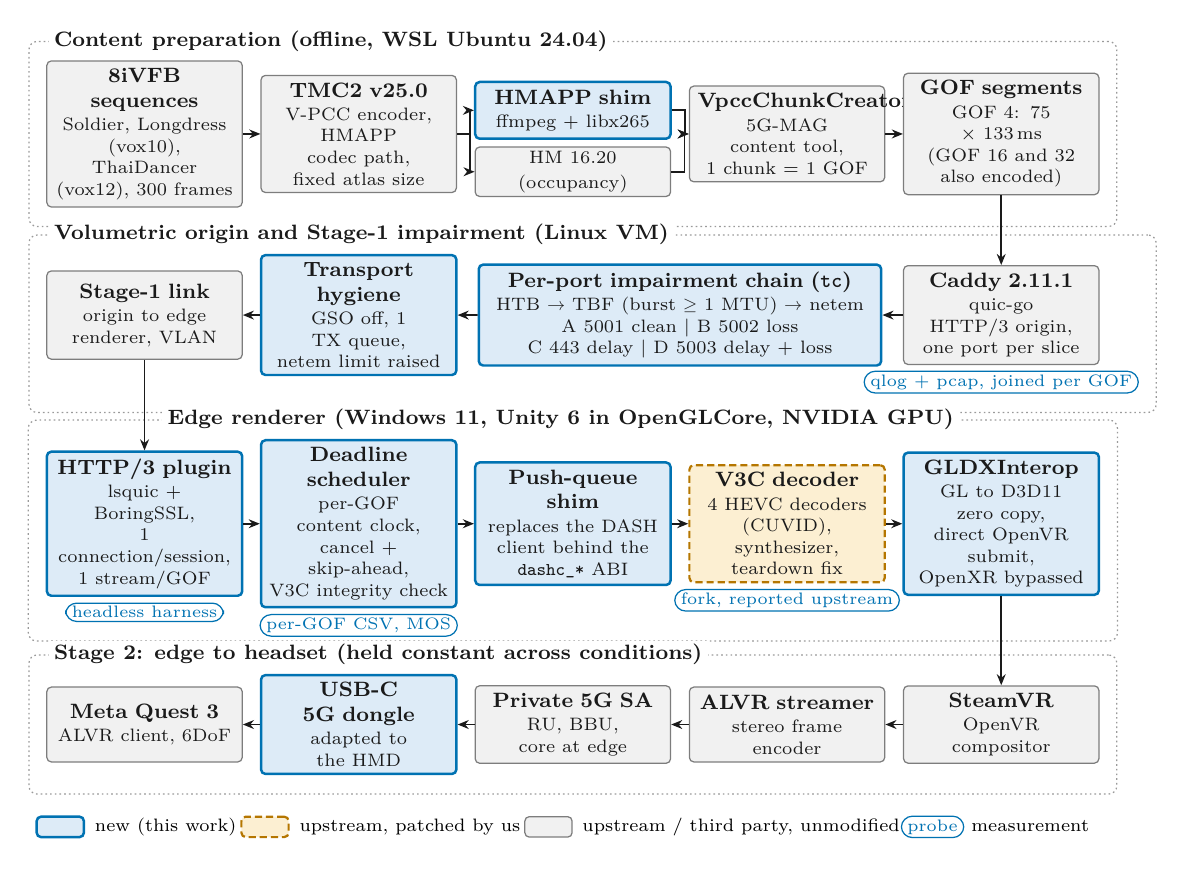
\begin{tikzpicture}[x=1cm,y=1cm]
  \def\xa{1.27}\def\xb{3.99}\def\xc{6.71}\def\xd{9.43}\def\xe{12.15}
  \tikzset{w/.style={text width=2.27cm, minimum height=1.12cm},
    probe/.style={font=\tinyfig, text=oiBlue, fill=white, draw=oiBlue,
      line width=0.45pt, rounded corners=4pt, inner xsep=2.2pt, inner ysep=1.2pt}}

  % ===================== lane 1: content preparation (L -> R) ==============
  \node[up, w] (pc) at (\xa,8.35) {\bx{8iVFB sequences}{Soldier, Longdress\\(vox10), ThaiDancer\\(vox12), 300 frames}};
  \node[up, w] (tmc) at (\xb,8.35) {\bx{TMC2 v25.0}{V-PCC encoder,\\HMAPP codec path,\\fixed atlas size}};
  \node[ours, w, minimum height=0.72cm] (shim) at (\xc,8.65) {\bx{HMAPP shim}{ffmpeg + libx265}};
  \node[up, w, minimum height=0.46cm, inner ysep=1.4pt] (hm) at (\xc,7.87) {{\smallfig HM 16.20 (occupancy)}};
  \node[up, w] (chunk) at (\xd,8.35) {\bx{VpccChunkCreator}{5G-MAG content tool,\\1 chunk = 1 GOF}};
  \node[up, w] (seg) at (\xe,8.35) {\bx{GOF segments}{GOF 4: 75 × 133\,ms\\(GOF 16 and 32\\also encoded)}};

  \draw[flow] (pc) -- (tmc);
  \draw[flow] (tmc.east) -- ++(0.17,0) |- (shim.west);
  \draw[flow] (tmc.east) -- ++(0.17,0) |- (hm.west);
  \draw[flow] (shim.east) -- ++(0.17,0) |- (chunk.west);
  \draw[flow] (hm.east) -- ++(0.17,0) |- (chunk.west);
  \draw[flow] (chunk) -- (seg);

  \begin{scope}[on background layer]
    \node[zone, fit=(pc)(tmc)(shim)(hm)(chunk)(seg), inner xsep=2.2mm,
      inner ysep=2.4mm] (z1) {};
  \end{scope}
  \node[zonetitle] at (z1.north west) {Content preparation (offline, WSL Ubuntu 24.04)};

  % ===================== lane 2: origin + stage-1 (R -> L) ==================
  \node[up, w] (caddy) at (\xe,6.05) {\bx{Caddy 2.11.1}{quic-go HTTP/3 origin,\\one port per slice}};
  \node[ours, text width=4.9cm, minimum height=1.12cm] (tc) at ($(\xc,6.05)!0.5!(\xd,6.05)$)
    {\bx{Per-port impairment chain (\code{tc})}{HTB $\rightarrow$ TBF (burst $\geq$ 1 MTU) $\rightarrow$ netem\\A 5001 clean \textbar{} B 5002 loss\\C 443 delay \textbar{} D 5003 delay + loss}};
  \node[ours, w] (hyg) at (\xb,6.05) {\bx{Transport hygiene}{GSO off, 1 TX queue,\\netem limit raised}};
  \node[up, w] (link) at (\xa,6.05) {\bx{Stage-1 link}{origin to edge\\renderer, VLAN}};
  \node[probe, anchor=north] (pr1) at ($(caddy.south)+(0,-0.07)$) {qlog + pcap, joined per GOF};

  \draw[flow] (seg) -- (caddy);
  \draw[flow] (caddy) -- (tc);
  \draw[flow] (tc) -- (hyg);
  \draw[flow] (hyg) -- (link);

  \begin{scope}[on background layer]
    \node[zone, fit=(caddy)(tc)(hyg)(link)(pr1), inner xsep=2.2mm,
      inner ysep=2.4mm] (z2) {};
  \end{scope}
  \node[zonetitle] at (z2.north west) {Volumetric origin and Stage-1 impairment (Linux VM)};

  % ===================== lane 3: edge renderer (L -> R) =====================
  \tikzset{w3/.style={text width=2.27cm, minimum height=1.42cm}}
  \node[ours, w3] (plg) at (\xa,3.4) {\bx{HTTP/3 plugin}{lsquic + BoringSSL,\\1 connection/session,\\1 stream/GOF}};
  \node[ours, w3] (sch) at (\xb,3.4) {\bx{Deadline scheduler}{per-GOF content clock,\\cancel + skip-ahead,\\V3C integrity check}};
  \node[ours, w3] (pq)  at (\xc,3.4) {\bx{Push-queue shim}{replaces the DASH\\client behind the\\\code{dashc\_*} ABI}};
  \node[mod, w3] (dec)  at (\xd,3.4) {\bx{V3C decoder}{4 HEVC decoders\\(CUVID), synthesizer,\\teardown fix}};
  \node[ours, w3] (gldx) at (\xe,3.4) {\bx{GLDXInterop}{GL to D3D11 zero copy,\\direct OpenVR submit,\\OpenXR bypassed}};
  \node[probe, anchor=north] (pr2) at ($(plg.south)+(0,-0.07)$) {headless harness};
  \node[probe, anchor=north] (pr3) at ($(sch.south)+(0,-0.07)$) {per-GOF CSV, MOS};
  \node[probe, anchor=north] (pr4) at ($(dec.south)+(0,-0.07)$) {fork, reported upstream};

  \draw[flow] (link.south) -- (plg.north);
  \draw[flow] (plg) -- (sch);
  \draw[flow] (sch) -- (pq);
  \draw[flow] (pq) -- (dec);
  \draw[flow] (dec) -- (gldx);

  \begin{scope}[on background layer]
    \node[zone, fit=(plg)(sch)(pq)(dec)(gldx)(pr2), inner xsep=2.2mm,
      inner ysep=2.4mm] (z3) {};
  \end{scope}
  \node[zonetitle] at ($(z3.north west)+(1.45,0)$) {Edge renderer (Windows 11, Unity 6 in OpenGLCore, NVIDIA GPU)};

  % ===================== lane 4: stage 2 (R -> L) ===========================
  \tikzset{w4/.style={text width=2.27cm, minimum height=0.95cm}}
  \node[up, w4] (svr)  at (\xe,0.85) {\bx{SteamVR}{OpenVR compositor}};
  \node[up, w4] (alvr) at (\xd,0.85) {\bx{ALVR streamer}{stereo frame encoder}};
  \node[up, w4] (fiveg) at (\xc,0.85) {\bx{Private 5G SA}{RU, BBU, core at edge}};
  \node[ours, w4] (dongle) at (\xb,0.85) {\bx{USB-C 5G dongle}{adapted to the HMD}};
  \node[up, w4] (q3) at (\xa,0.85) {\bx{Meta Quest 3}{ALVR client, 6DoF}};

  \draw[flow] (gldx) -- (svr);
  \draw[flow] (svr) -- (alvr);
  \draw[flow] (alvr) -- (fiveg);
  \draw[flow] (fiveg) -- (dongle);
  \draw[flow] (dongle) -- (q3);

  \begin{scope}[on background layer]
    \node[zone, fit=(svr)(alvr)(fiveg)(dongle)(q3), inner xsep=2.2mm,
      inner ysep=2.4mm] (z4) {};
  \end{scope}
  \node[zonetitle] at (z4.north west) {Stage 2: edge to headset (held constant across conditions)};

  % ===================== legend ==============================================
  \provlegend{0.2,-0.45}
  \node[anchor=west, font=\smallfig] at (10.75,-0.45)
    {\tikz[baseline=-0.6ex]\node[probe]{probe};\ measurement};
\end{tikzpicture}
\end{document}
